\chapter{Odhad kopula funkce}

Koncept kopule zahrnuje několik podkladových funkcí - marginální distribuční funkce jednotlivých náhodných veličin a kopula funkci, která popisuje závilost jejich kvantilů. Protože volba marginální funkce má skrze jí implikované kvantily vliv na volbu kopula funkce, měly by se teoreticky obě odhadovat společně. To je však v praxi poměrně obtížné, a proto odhad zpravidla probíhá ve dvou krocích - v prvním kroku se odhadnou marginální distribuční funkce a ve druhém kroku se hledá kopula funkce, která nejlépe odpovídá kvantilům, které byly vypočteny na základě jednotlivých distribučních funkcí.

\begin{figure}[htp]
\centering
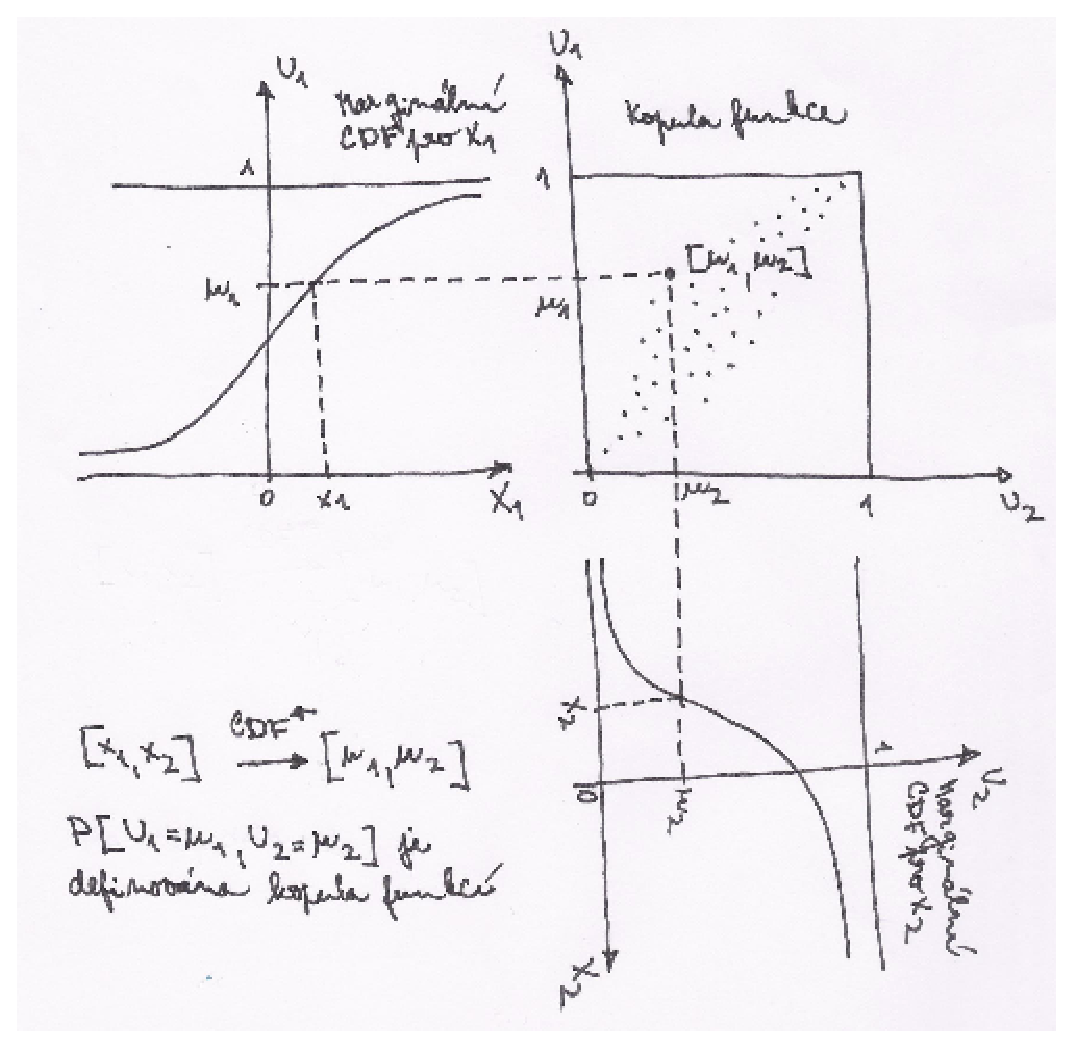
\includegraphics[scale = 0.50]{pictures/copula_concept.eps}
\caption{Koncept kopula funkce}
\end{figure}

\section{Marginální distribuční funkce}

Prvním krokem je odhad marginálních distribučních funkcí, z nichž následně odvodíme kvantily pro jednotlivá pozorování. Marginální distribuční funkce je možné odhadnout několika různými způsoby. Mezi nejběžnější patří následující.
\begin{itemize}
\item Nejjednodušším způsobem je aproximace pomocí empirické distribuční funkce. Nevýhodou tohoto přístupu je, že (a) odhadnutá distribuční funkce je nespojitá, což představuje problém při její inverzi a (b) z důvodu nedostatečného počtu extrémních pozorování nemusí správně odhadovat odlehlé kvantily.
\item Další neparametrický způsob odhadu distribuční funkce spočívá ve využitím jádrového vyhlazení (kernel smoothing) empirických dat. Tento přístup je tedy rozšířením předhozího. Distribuční funkce je, zjednodušeně řečeno, v jednotlivých bodech odhadu aproximována pomocí váženého průměru jednotlivých empirických kvantilů. Výhodou oproti předchozímu přístupu je hladká distribuční funkce, nicméně problém s odlehlými kvantily zůstává.
\item Právě z důvodu problému s odlehlými kvantily je preferován parametrický odhad. V tomto případě se zvolí konkrétní pravděpodobnostní rozdělení, jehož parametry se následně odhadnou na základě empirických dat. Výhodou je hladká distribuční funkce, pro kterou máme zpravidla k dispozici funkční předpis. Na druhou stranu právě z důvodu volby pravděpodobnostního rozdělení zahrnuje tento postup určitou míru subjektivity.
\end{itemize}

Než se zaměříme na jednotlivé způsoby odhadu distribuční funkce, je třeba zdůraznit, že volba marginální distribuční funkce má dopad na výpočet hodnoty kvantilů a tím pádem také na následný odhad kopula funkce. Nevhodný způsob konstrukce marginální distribuční funkce tak může mít fatální důsledky.

\subsection{Empirická distribuční funkce}

Předpokládejme, že máme k dispozici určitý počet pozorovaných hodnot z realizace náhodné veličiny jako je např. logaritmická změna ceny konkrétní akcie obchodované na burze v průběhu určitého období.

Prvním krokem při konstrukci empirické distribuční funkce je rozdělení reálné osy (tj. v našem případě možného cenového rozpětí) na několik disjuktních intervalů. Jejich počet závisí na počtu pozorování, která máme k dispozici - čím více pozorování, tím více může být těchto intervalů. Každé pozorování přiřadíme  s ohledem na jeho hodnotu právě jednomu z těchto intervalů.

Po té, co máme všechna pozorování přiřazena, spočítáme jejich relativní četnost pro jednotlivé intervalech. Délka intervalů nemusí být shodná - v ideálním případě by měla být nastavena tak, aby každý z nich obsahoval přibližně stejný počet pozorování. Tím omezíme velikost ``schodů'' empirické distribuční funkce při přechodu z jednoho intervalu do druhého.

Posledním krokem je postupné načítání relativních četností přes jednotlivé intervaly, čímž získáme empirickou distribuční funkci. Tato funkce je nespojitá, tj. vykazuje ``schody'' při přechodu z jednoho intervalu do druhého. Ačkoliv lze velikost těchto ``schodů'' omezit navýšením počtu pozorování (a s tím souvisejícím větším počtem možných intervalů) popř. vhodnou volbou intervalů (viz. výše), zcela zbavit se jich nelze. Nespojitost empirické distribuční funkce znamená, že neexistuje její inverzní funkce, což je třeba zohlednit při případné simulaci.

Je zřejmé, že kvalita empirické distribuční funkce je silně závislá na počtu pozorování. To platí zejména pro odlehlé kvantily. Jestliže máme např. k dispozici 100 pozorování, nemůžeme na základě empirické distribuční funkce vznášet závěry ohledně kvantilu 0.1\% a 99.9\%. A právě tyto kvantily jsou hlavním předmětem zájmu při řízení finančních rizik, což snižuje použitelnost tohoto přístupu v praxi.

\subsection{Jádrové vyhlazení}

\subsubsection{Popis metody}

Jádrové vyhlazení je statistická technika pro odhad reálné funkce $f(X), X \in R^d$ na základě empirických dat v případech, kdy není znám funkční předpis $f(x)$. Odhadovaná funkce je hladká, přičemž stupeň ``vyhlazení'' je dán jediným parametrem.

Nechť $K_{h_{\lambda}}(X_0, X)$ je jádro definované jako
\begin{equation*}
K_{h_{\lambda}}(X_0, X) = D\left(\frac{\parallel X - X_0\parallel}{h_{\lambda}(X_0)} \right)
\end{equation*}
kde $X, X_0 \in R^d$, $h_{\lambda}(X_0)$ je parametr vyhlazení a $D(t)$ je kladná reálná funkce, jejíž hodnota klesá s rostoucím $\parallel X - X_0\parallel$, tj. vzdáleností mezi body $X$ a $X_0$.
Nechť $\hat{Y}(X): R^d \rightarrow R$ je spojitou funkcí proměnné $X$. Pak pro libovolné $X_0 \in R^d$ je Nadaraya-Watsonův vážený průměr založený na jádře definován jako
\begin{equation*}
\hat{Y}(X_0) = \frac{\sum_{i = 1}^N K_{h_{\lambda}}(X_0, X_i)Y(X_i)}{\sum_{i = 1}^N K_{h_{\lambda}}(X_0, X_i)}
\end{equation*}
kde $N$ je počet pozorování a $Y(X_i)$ je hodnota pozorování v bodě $X_i$.

Existuje řada jader, nicméně nejčastěji používaným je Gausovo jádro. To je definováno jako
\begin{equation*}
K_{h_{\lambda}}(X_0, X) = \frac{1}{\sqrt{2 \pi h^2}} e^{-\frac{1}{2}\left(\frac{\parallel X - X_0\parallel}{h}\right)^2}
\end{equation*}
kde parametr vyhlazení je zpravidla zvolen jako $h = 1.06 \sigma_Y N ^{-\frac{1}{5}}$ s $\sigma_Y$ představující směrodatnou odhylku hodnot pozorování $Y(X_i)$. 

\subsubsection{Aplikace}

Po té, co je na základě pozorování zkonstruována empirická distribuční funkce, lze na tuto funkci aplikovat jádrové vyhlazení. Výhodou jádrového vyhlazení je, že lze empirickou distribuční funkci tabularizovat na libovolně husté stupnici, čímž lze zásadním způsobem eliminovat problém ``schodů''. Výsledná tabulka se následně používá pro inverzi distribuční funkce. Funkce \textit{KernelSmoothing.m} jádrové vyhlazení je k dispozici v adresáři \textit{libs}. 

\begin{figure}[htp]
\centering
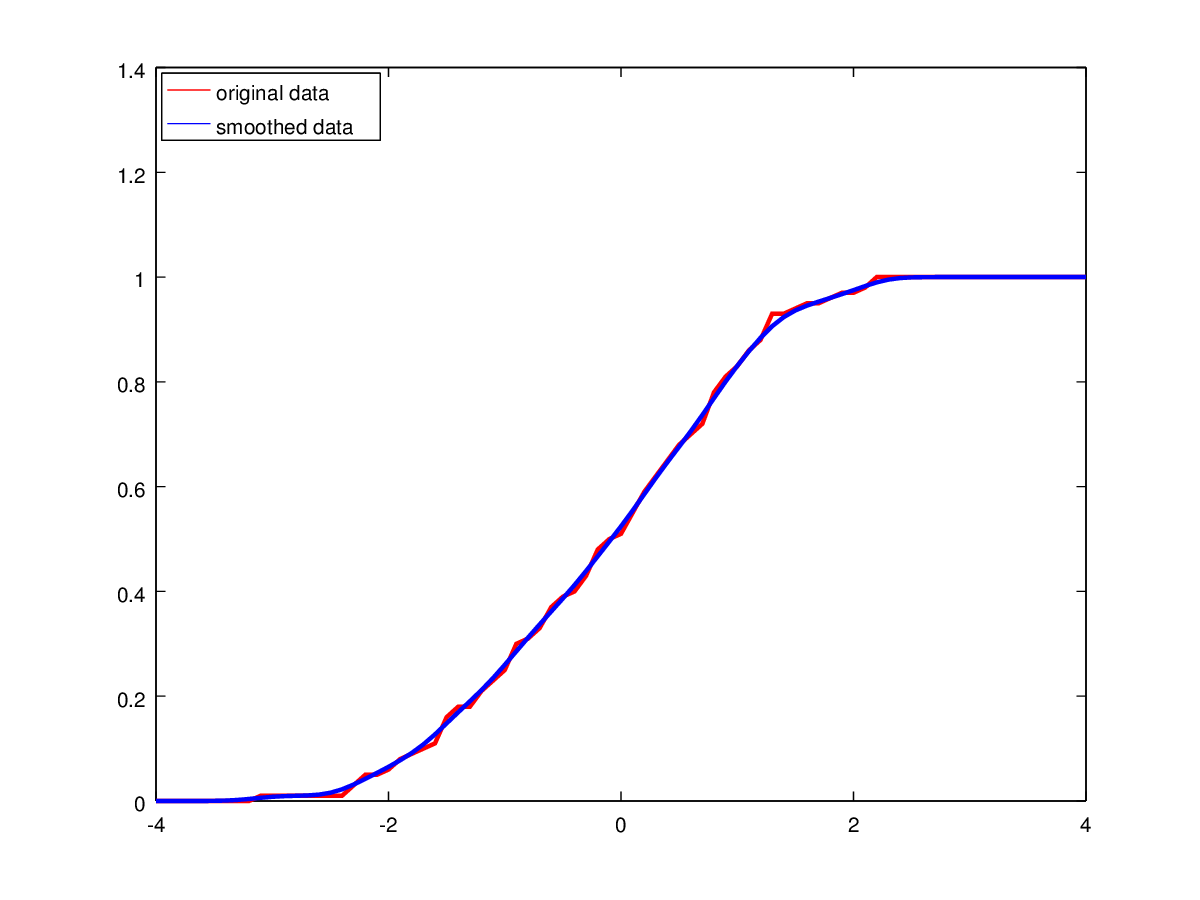
\includegraphics[scale = 0.50]{pictures/kernel_smoothing.eps}
\caption{Vyhlazená empirická distribuční funkce}
\end{figure}

\subsection{Volba pravděpodobnostního rozdělení}

Ve finační teorii se velmi často používá vybraná rodina pravděpodobnostních rozdělení pro popis chování určitých finanční veličin. Nejpopulárnější je normální rozdělení, které se používá pro popis logaritmických změn cen akcií a měnových kurzů nebo absolutních změn úrokových sazeb a spreadů. Namísto normálního rozdělení se často používá také studentovo rozdělení, které je do určité míry schopné modelovat tlusté chvosty. Společnou nevýhodou normálního a studentova rozdělení je jejich symetrie kolem střední hodnoty, která není pro finanční data příliš typická.

Vedle těchto běžných rozděleních se používá také řada exotičtějších rozdělení. Jako příklad uveďme variance-gamma rozdělení, které vedle tlustých konců modeluje také skokové změny (např. náhlý propad cen), a proto se používá především pro modelování cen akcií. Dalším často používaným je také GEV (generalized extreme value) pravděpodobnostní rozdělení, které řeší problém tlustých chvostů a symetrie pravděpodobnostního rozdělení (avšak není schopné modelovat případné skokové změny ve finančních datech).

Prvním a zásadním krokem je tedy, s ohledem na charakter modelované finanční veličiny, vybrat vhodné pravděpodobnostní rozdělení. Druhým krokem je odhad parametrů zvoleného pravděpodobnostního rozdělení na datech, které máme k dispozici. Vždy je vhodné alespoň vizuálně porovnat odhadnuté pravděpodobnostní rozdělení s původními daty.

\subsubsection{Normální rozdělení}

Odhad parametrů v případě normálního rozdělení je triviální - stačí spočítat střední hodnotu $\mu$ resp. směrodatnou odchylku $\sigma$ z dat dané finanční veličiny jako

\begin{equation*}
\mu = \frac{\sum_{i = 1}^N x_i}{N}
\end{equation*}
resp.
\begin{equation*}
\sigma = \sqrt{\frac{\sum_{i = 1}^N(x_i - \mu)}{N - 1}}
\end{equation*}
kde $N$ představuje počet pozorování, která máme k dispozici.

\subsubsection{Studentovo rozdělení}

V případě studentova rozdělení je třeba odhadnout také počet stupňů volnosti. Navíc rozptyl je funkcí počtu stupňů volnosti, což odhad parametrů poněkud komplikuje. Na druhou stranu tento parametr umožnuje lepší podchycení případných tlustých chvostů, které jsou typické pro finanční data.

Uvažujme náhodnou veličinu $X$, pro kterou budeme odhadovat parametry studentova rozdělení. Narozdíl od normálního rozdělení se parametry studentova rozdělení odhadují iterativně. Před samotnou iterací je však třeba nejprve vypočíst počáteční odhad střední hodnoty $\mu_{ini} = \frac{\sum_{i = 1}^N x_i}{N}$ a  počáteční odhad rozptylu $\sigma^2_{ini} = \frac{\sum_{i=1}^N \tilde{x}_i^2}{N - 1}$, kde $x_i$ představuje hodnotu $i$-tého pozorování náhodné veličiny $X$ a $N$ celkový počet pozorování. Dále je třeba arbitrárně stanovit počáteční odhad pro počet stupňů volnosti $\nu_{ini}$. Výpočet parametrů studentova rozdělení pak probíhá podle následujících kroků.
\begin{enumerate}
\item Předpokládejme, že pro $t$-tou iteraci je stanoven počet stupňů volnosti $\nu(t)$ - $\nu(1)$ je rovno počátečnímu odhadu $\nu_{ini}$; pro $t > 1$ je $\nu(t)$ výstupem předchozí iterace.
\item Krok E1
\begin{enumerate}
\item Vypočteme tzv. Mahalanobisovu vzdálenost pozorování $x_i$ od $\mu$ vzhledem k rozptylu $\Psi(t)$ jako
\begin{equation*}
\delta_i(t) = \frac{(x_i - \mu(t))^2}{\Psi(t)}
\end{equation*}
kde $\mu(1) = \mu_{ini}$ a $\Psi(1) = \sigma^2_{ini}$; pro $t > 1$ jsou $\mu(t)$ a $\Psi(t)$ výstupem předešlé iterace.
\item Mahalanobisova vzdálenost $\delta_i(t)$ je vstupem pro následný výpočet vah.
\begin{equation*}
w_{i}(t) = \frac{\nu(t) + 1}{\nu(t) + \delta_i(t)}
\end{equation*}
\item S pomocí vah $w_{i}(t)$ vypočteme níže uvedené dostatečné statistiky.
\begin{gather*}
S_{\tau}(t) = \sum_{i = 1}^N w_i(t)\\
S_{\tau X}(t) = \sum_{i = 1}^N w_i(t)x_i\\
S_{\tau XX}(t) = \sum_{i = 1}^N w_i(t)x_i^2
\end{gather*}
\end{enumerate}
\item Krok CM1
\begin{enumerate}
\item Zaktualizujeme odhad střední hodnoty.
\begin{equation*}
\mu(t) = \frac{S_{\tau X}(t)}{S_{\tau}(t)}
\end{equation*}
\item Zaktualizujeme odhad rozptylu.
\begin{equation*}
\Psi(t) = \frac{1}{N}\Big(S_{\tau XX}(t + 1) - \frac{1}{S_{\tau (t)}S_{\tau X}^2}\Big)
\end{equation*}
\end{enumerate}
\item Krok E2 - Přepočteme váhy $w_i(t)$ a dostatečné statistiky $S_{\tau}(t)$, $S_{\tau X}(t)$, $S_{\tau XX}(t)$ s ohledem na zaktualizovanou střední hodnotu $\mu(t)$ a rozptyl $\Psi(t)$ (viz. krok E1).
\item Krok CM2
\begin{enumerate}
\item Zaktualizujeme odhad počtu stupňů volnosti řešením rovnice
\begin{equation*}
-\phi\big(\frac{v}{2}\big) + \ln \big(\frac{v}{2}\big) + \frac{1}{N}\sum_{i = 1}^N \Big(\ln(w_i(t)) - w_i(t)\Big)
\end{equation*}
pro $v$, kde $\phi(x) = \frac{d \ln(\Gamma(x))}{dx}$ je tzv. digamma funkce.
\item Přepočteme váhy s ohledem na zaktualizovaný odhad počtu stupňů volnosti.
\begin{equation*}
w_i = \frac{v(t) + 1}{v(t) + \delta_i(t)}
\end{equation*}
\end{enumerate}
\item Pokud změny parametrů $\mu(t)$, $\nu(t)$ a $\Psi(t)$ oproti iteraci $t-1$ překračují námi stanovéné meze, pokračuje v iteraci přesunem na bod (1). V opačném případě považujeme odhad parametrů za dostatečně přesný a iteraci ukončíme.
\end{enumerate}

Funkce \textit{StudentFit.m} pro odhad parametrů studentova rozdělení je k dispozici v adresáři \textit{libs}.

\section{Kopula funkce}

Po odhadu marginálních distribučních funkcí a převedení hodnot jednotlivých pozorování na kvantily je možné přistoupit k odhadu kopula funkce.

Stejně jako v případě marginální distribuční funkce je možné kopula funkci odhadnout empiricky a popř. tento empirický odhad dále jádrově vyhladit. Nicméně v praxi má odhad nejčastěji podobu odhadu parametrů konkrétní kopula funkce. V následujícím textu se budeme zabývat dvourozměrnou Gausovou, studentovou, Claytonovou, Frankovou a Gumbelovou kopula funkcí. To, která konkrétní kopula funkce je v daném případě nejvhodnější, se často posuzuje vizuálně.

\subsection{Gausova kopula funkce}

Gausova kopule je pro svou relativní jednoduchost nejčastěji používanou kopula funkcí.

\begin{figure}[htp]
\centering
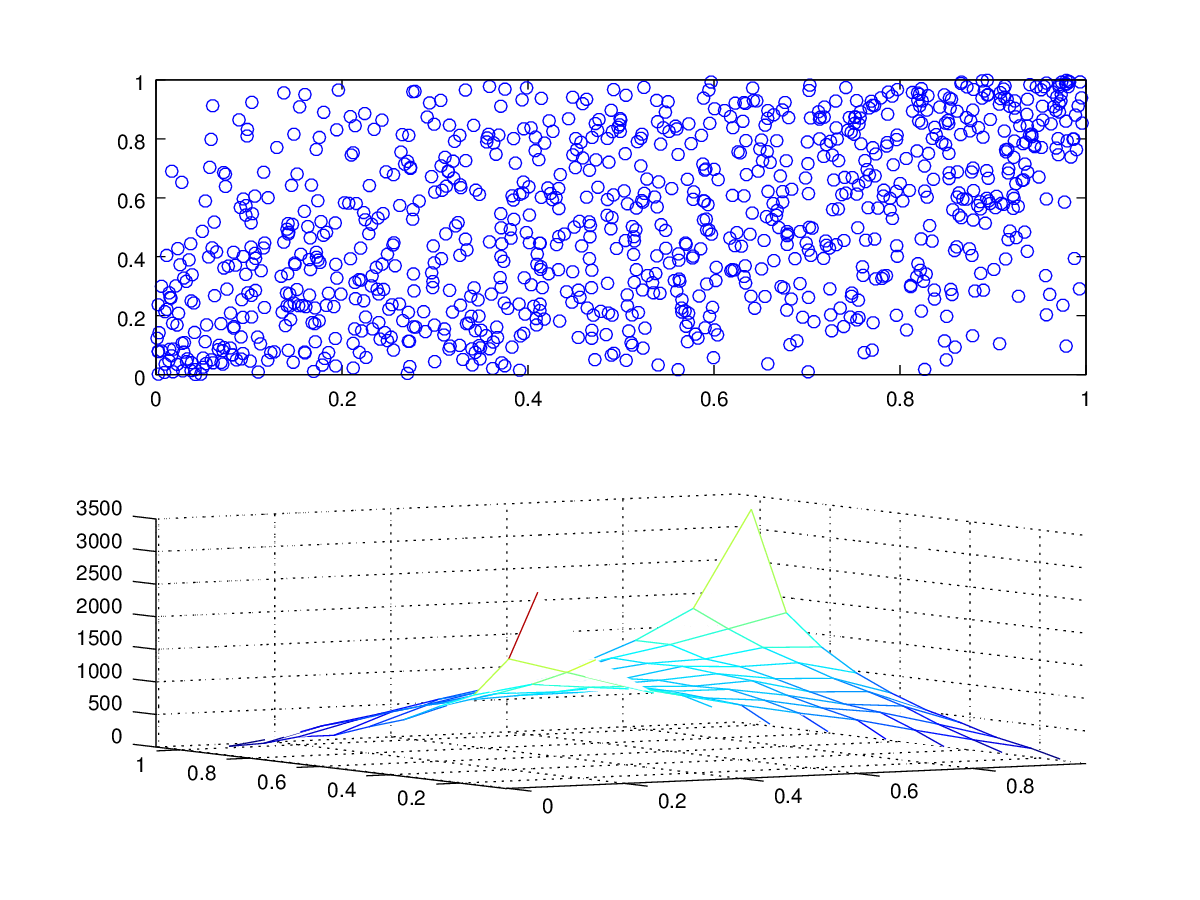
\includegraphics[scale = 0.50]{pictures/gaussian.eps}
\caption{Dvourozměrná Gausova kopula funkce s korelačním parametrem $\rho =   0.5$}
\end{figure}

\subsubsection{Odhad parametrů}

Gausova kopula je plně definována korelační maticí. Tu lze odhadnout pomocí Kendall pořadové korelace, kterou lze převést na klasickou korelaci $\rho$ pomocí vztahu
\begin{equation*}
\rho(X) = \sin\left(\frac{\pi}{2}\right)
\end{equation*}
Z jednotlivých párových korelací pak lze sestavit kompletní korelační matici. Takto zkonstruovaná matice nemusí být nutně pozitivně semidefinitní (i když tomu tak v praxi obvykle bývá), a proto je vhodné provést kontrolu a matici případně upravit.

Související funkce \textit{CalcKendallTau.m} je k dispozici v adresáři \textit{libs}.

Funkce \textit{FitGausianCopula.m} pro odhad parametrů Gausovy kopula funkce je k dispozici v adresáři \textit{Copulas}.

\subsubsection{Simulace}

Předpokládejme, že máme k dispozici korelační matici $\Sigma$, kterou jsme odhadli v předchozím kroku.

\begin{enumerate}
\item Pomocí Choleskyho dekompozice provedeme rozklad kovarianční matice na $\Sigma = \Sigma^{1/2} \Sigma^{1/2}$.
\item Vygenerujeme vektor $Z = (Z_1, Z_2, ..., Z_d)' \sim N(0, \Sigma)$ nezávislých standardních normálních veličin.
\item Vypočteme vektor $X = \Sigma^{1/2}Z$ korelovaných standardních normálních veličin, kde $X = (X_1, X_2, ..., X_d)$.
\item Vypočteme $U = \left(\Phi(X_1), \Phi(X_2), ..., \Phi(X_d)) \right)$, kde $\Phi$ je distribuční funkce standardního normálního rozdělení. Náhodný vektor $U$ sleduje Gausovu kopula funkci\footnote{Připomeňme, že Gausova kopula funkce je distribuční funkcí. Vektor $U$ tak lze chápat jako náhodný výběr z této distribuční funkce. To je ostatně smyslem výše popsané simulace.}.
\end{enumerate}

Související funkce \textit{SimulGausianCopula.m} je k dispozici v adresáři \textit{Copulas}.

\subsubsection{Asymptotická nezávislost ve chvostech}

Nechť $(X_1, X_2) := (\Phi^{-1}(U_1), \Phi^{-1}(U_2))$ tak, že $(X_1, X_2)$ sleduje dvourozměrné normální rozdělení se standardním normálním rozdělením jako marginální distribuční funkcí a korelací $\rho$. Koeficient závislosti v dolním chvostu této Gaussovy kopula funkce je
\begin{multline*}
\lambda = 2 \lim_{x \rightarrow 0^+} P(\Phi^{-1}(U_2) \le \Phi^{-1}(q) | \Phi^{-1}(U_1) = \Phi^{-1}(q))\\
= 2 \lim_{x \rightarrow -\infty} P(X_2 \le x | X_1 = x)
\end{multline*}
S využitím skutečnosti $X_2 | X_1 = x \sim N(\rho x, 1 - \rho^2)$\footnote{Nechť $X_1$ a $X_2$ jsou dvě nezávislé náhodné veličiny, které sledují standardizované normální rozdělení. Definujme $\epsilon_1 = X_1$ a $\epsilon_2 = \rho X_1 + \sqrt{1 + \rho^2}X_2$. Lze dokázat, že $\epsilon_1$ a $\epsilon_2$ jsou náhodné veličiny s korelací $\rho$, které sledují standardizované normální rozdělení. Platí
\begin{equation*}
E[\epsilon_2 | \epsilon_1 = \epsilon^*] = E[\rho \epsilon^* + x_2 \sqrt{1 - \rho^2}] = \rho \epsilon^*
\end{equation*}
\begin{equation*}
E[\epsilon_2^2 | \epsilon_1 = \epsilon^*] = E[(\rho \epsilon^*)^2 + 2 \rho \epsilon^* x_2(1 - \rho^2) + (1 - \rho^2)x_2^2] = (\rho \epsilon^*)^2 + (1 - \rho^2)
\end{equation*}
což implikuje
\begin{multline*}
D[\epsilon_2 | \epsilon_1 = \epsilon^*] = E[\epsilon_2^2 | \epsilon_1 = \epsilon^*] - E[\epsilon_2 | \epsilon_1 = \epsilon^*]^2\\
= (\rho \epsilon^*)^2 + (1 - \rho^2) - (\rho \epsilon^*)^2 = 1 - \rho^2
\end{multline*}
a proto $\epsilon_2 | \epsilon_1 = \epsilon^* \sim N(\rho \epsilon^*, 1 - \rho^2)$.} lze odvodit
\begin{equation*}
P(X_2 \le x | X_1 = x) = \Phi\left(\frac{x - \rho x}{\sqrt{1 - \rho^2}} \right) = \Phi \left(\frac{x \sqrt{1 - \rho}^2}{\sqrt{1 - \rho}\sqrt{1 + \rho}}\right) = \Phi \left(\frac{x \sqrt{1 - \rho}}{\sqrt{1 + \rho}} \right)
\end{equation*}
a proto
\begin{equation*}
\lambda = 2 \lim_{x \rightarrow -\infty} \Phi\left(\frac{x \sqrt{1 - \rho}}{\sqrt{1 + \rho}}\right) = 0
\end{equation*}
za předpokladu $\rho < 1$. Gausova kopula funkce je tedy asymptoticky nezávislá v obou chvostech a to bez ohledu na to, jak vysokou korelaci $\rho$ zvolíme.

\subsubsection{Omezení}

Ačkoliv je Gausova kopula funkce jednou z nejpoužívanějších, má řadu zásadních omezení.

Gausova kopula funkce patří do rodiny eliptických funkcí - jedná se tedy o symetrickou distribuční funkci. To znamená, že např. pravděpodobnost extrémního nárůstu cen akcií je shodná s pravděpodobností extrémně negativního poklesu. To je v rozporu s empirickým pozorováním, kdy pravděpodobnost extrémního poklesu je zpravidla výrazně vyšší než pravděpodobnost extrémního nárůstu.

Notoricky známým nedostatkem normálního rozdělení je nedostatečné podchycení případných tlustých chvostů. Z empirických dat je zřejmé, že právě tlusté chvosty jsou typická pro finanční data.

Jak jsme ukázali výše, dalším zásadním nedostatkem je skutečnost, že korelace mezi jednotlivými náhodnými veličinami se v chvostech Gausovy kopula funkce asymptoticky blíží nule. Pokud je tedy předmětem našeho zájmu vypočet value-at-risk, který se opírá o kvantily 99\% a vyšší, je Gausova kopula funkce nevhodná.

\subsection{Studentova kopula funkce}

Narozdíl od Gausovy kopula funkce umožňuje studentova kopula funkce částečně podchytit problematiku tlustých chvostů a to skrze parametr počet stupňů volnosti. Nicméně standardní studentova kopula funkce má pouze jeden takovýto parametr bez ohledu na dimenzi $d$. Podobně jako pro Gausovu kopula funkci jsou parametry studentovy kopula funkce relativně snadno odhadnutelné, což je jeden z hlavních důvodů její oblíbenosti v praxi.

\begin{figure}[htp]
\centering
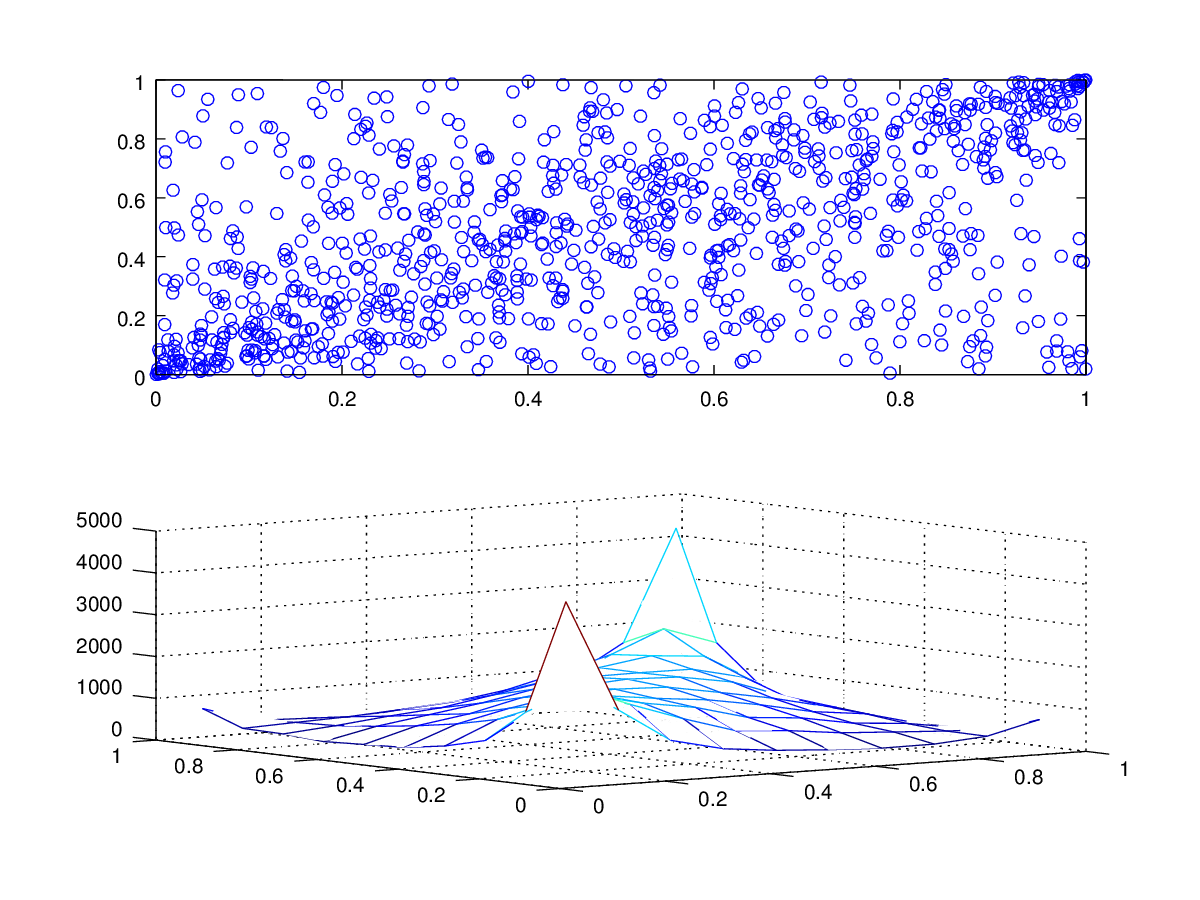
\includegraphics[scale = 0.50]{pictures/student.eps}
\caption{Dvourozměrná studentova kopula funkce s korelačním parametrem $\rho =   0.5$ a počtem stupňů volnosti $\nu = 2$}
\end{figure}

\subsubsection{Odhad parametrů}

V případě studentovy kopula funkce je třeba odhadnout kromě korelační matice také počet stupňů volnosti. Stejně jako v případě Gausovy kopula funkce lze korelační matice odhadnout pomocí Kendall pořadové korelace. Počet stupňů volnosti lze odhadnout pomocí MLE maxilizací funkce
\begin{equation*}
\max_{\nu} \sum_{i = 1}^N \ln \Big(c_{\nu, \Sigma}^t(u_i)\Big)
\end{equation*}
kde $u_i$ představuje vektor dimenze $d$ obsahující kvantily $i$-tého pozorování, $N$ představuje celkový počet pozorování a $c_{\nu, \Sigma}^t(u_i)$ je hustotu pravděpodobnosti studentovy kopula funkce definovanou jako
\begin{equation*}
c_{\nu, \Sigma}^t(u_i) = \frac{f_{\nu, \Sigma}(t_{v}^{-1}(u_{i1}), t_{v}^{-1}(u_{i2}), ..., t_{v}^{-1}(u_{id}))}{\prod_{j = 1}^d f_{\nu}(t_{\nu})^{-1}(u_{ij})}, ~~~ u \in (0, 1)^d
\end{equation*}
kde $f_{\nu, \Sigma}$ je sdružená hustota pravděpodobnosti $d$-rozměrného studentova rozdělení s $\nu$ stupni volnosti a korelační maticí $\Sigma$ a $f_{\nu}$ je hustota pravděpodobnosti jednorozměrného studentova rozdělení s $\nu$ stupni volnosti. 

Funkce \textit{FitStudentCopula2.m} pro odhad parametrů studentovy kopula funkce je k dispozici v adresáři \textit{Copulas}.

\subsubsection{Simulace}

Předpokládejme, že máme k dispozici korelační matici $\Sigma$ a počet stupňů volnosti, které jsme odhadli v předchozím kroku.

\begin{enumerate}
\item Pomocí Choleskyho dekompozice provedeme rozklad kovarianční matice na $\Sigma = \Sigma^{1/2} \Sigma^{1/2}$.
\item Vygenerujeme vektor $Z = (Z_1, Z_2, ..., Z_d)' \sim N(0, \Sigma)$ nezávislých standardních normálních veličin.
\item Vypočteme vektor $X = \Sigma^{1/2}Z$ korelovaných standardních normálních veličin, kde $X = (X_1, X_2, ..., X_d)$.
\item Vygenerujeme náhodnou veličinu $Y$ z $\chi^2$ pravděpodobnostního rozdělení s parametrem $\nu$.
\item Vypočteme vektor $T = \left( \frac{X_1}{\nu / \sqrt{Y}}, \frac{X_2}{\nu / \sqrt{Y}}, \frac{X_d}{\nu / \sqrt{Y}} \right)$.
\item Vypočteme $U = \left(t_{\nu}^{cdf}(T_1), t_{\nu}^{cdf}(t_2), ...,  t_{\nu}^{cdf}(Z_d)) \right)$, kde $t_{\nu}^{cdf}$ je distribuční funkce studentova rozdělení s $\nu$ stupni volnosti. Náhodný vektor $U$ sleduje studentovu kopula funkci s korelační maticí $\Sigma$ a $\nu$ stupni volnosti.
\end{enumerate}

Související funkce \textit{SimulStudentCopula.m} je k dispozici v adresáři \textit{Copulas}.

\subsubsection{Asymptotická závislost v chvostech}

Uvažujme $(X_1, X_2) := (t_{\nu}^{-1}(U_1), t_{\nu}^{-1}(U_2))$, kde $t_{\nu}$ označuje distribuční funkci jednorozměrného studendova rozdělení s $\nu$ stupni volnosti. Proto $(X_1, X_2) \sim t_2(\nu, 0, P)$, kde $P$ je korelační matice s prvkem $\rho$ mimo hlavní diagonálu. Lze dovodit, že podmíněná pravděpodobnost pro $X_1 = x$ zdvourozměrného studentova rozdělení je
\begin{equation*}
\left(\frac{v + 1}{v + x^2}\right)^{\frac{1}{2}} \frac{X_2 - \rho x}{\sqrt{1 - \rho^2}} \sim t_{v + 1}
\end{equation*}
Podobnou argumentací jako v případě Gausovy kopula funkce lze dokázat
\begin{equation*}
\lambda = 2 t_{v + 1} \left(-\sqrt{\frac{(v + 1)(1 - \rho)}{1 + \rho}}\right)
\end{equation*}
Za předpokladu $\rho > - 1$ tedy studentova kopula funkce vykazuje závislost ve svém horním i dolním chvostu.

\subsubsection{Omezení}

Na studentovu kopula funkci lze pohlížet jako na zobecnění Gausovy kopula funkce. Přesto (anebo spíše právě proto) sdílí s Gausovou kopula funkcí řadu omezení.

Stejně jako Gausova kopula funkce patří studentova kopula funkce do rodiny eliptických funkcí a jedná se tedy o symetrickou distribuční funkci. Empirická data však hypotézu o symetrii příliš nepodporují. Tomuto problému se lze vyhnout pomocí tzv. sešikmené studentovy kopula funkce, která je rozšířením původního modelu. Odhad parametrů sešikmení je však časově poměrně náročný.

Tlusté chvosty jsou částečně podchyceny skrze počet stupňů volnosti. Nicméně základní studentova kopula funkce má pouze jeden takovýto parametr bez ohledu na svou dimenzi. Problém lze částečně obejít rozšířením modelu, kdy pro každou dimenzi definujeme vlastní počet stupňů volnosti - hovoříme o tzv. studentově kopula funkcí s vícero stupni volnosti. Kalibrace této kopula funkce je však časově náročná, a proto se v praxi příliš nepoužívá. Funkce \textit{FitStudentMDoF.m} a \textit{SimulStudentMDoF.m}, které slouží ke kalibraci resp. k simulaci tohoto typu kopula funkce jsou k dispozici v adresáři \textit{Copulas}.

Na rozdíl od Gausovy kopula funkce se korelace v chvostech asymptoticky neblíží nule. To však neznamená, že modelová korelace odpovídá skutečné korelaci. Teoretickým řešením je sloučení dvou výše uvedených rozšíření v tzv. sešikmenou studentovu kopula funkci s vícero stupni volnosti, kdy skrze větší počet parametrů získáme potřebnou flexibilitu. V praxi však tento přístup naráží na problém s kalibrací, která je nestabilní a navíc velmi časově náročná.

\subsection{Archimediánské kopula funkce}

Obecná Archimediánská kopula funkce je definována jako
\begin{equation}
C(u_1, u_2) = \phi^{-1}\left(\phi(u_1) + \phi(u_2)\right)
\end{equation}
kde $\phi$ je klesající funkce, která mapuje z $[0, 1]$ do $[0, \infty]$ a splňuje $\phi(0) = \infty$ a $\phi(1) = 0$. Funkci $\phi$ nazýváme kopula generátorem. Z (2.1) vyplývá, že Archimediánské kopule jsou dvourozměrné. Existují také vícerozměrné varianty Archimediánských kopula funkcí, ty však nejsou předmětem tohoto textu. Do rodiny Archimediánských kopula funkcí patří Claytonova, Gumbelova a Frankova kopula funkce.

\subsubsection{Claytonova kopula funkce}

Dvourozměrná Claytonova kopula funkce má tvar
\begin{equation*}
C_{\theta}(u_1, u_2) = (u_1^{-\theta} + u_2^{-\theta} - 1)^{-\frac{1}{\theta}}, ~~~ 0 < \theta < \infty
\end{equation*}
Pro $\theta \rightarrow 0$ získáme nezávislou kopula funkci; pro $\theta \rightarrow \infty$ získáme komonotonickou kopula funkci. Parametr $\theta$ tak měří sílu závislosti v rámci kopula funkce.

\begin{figure}[htp]
\centering
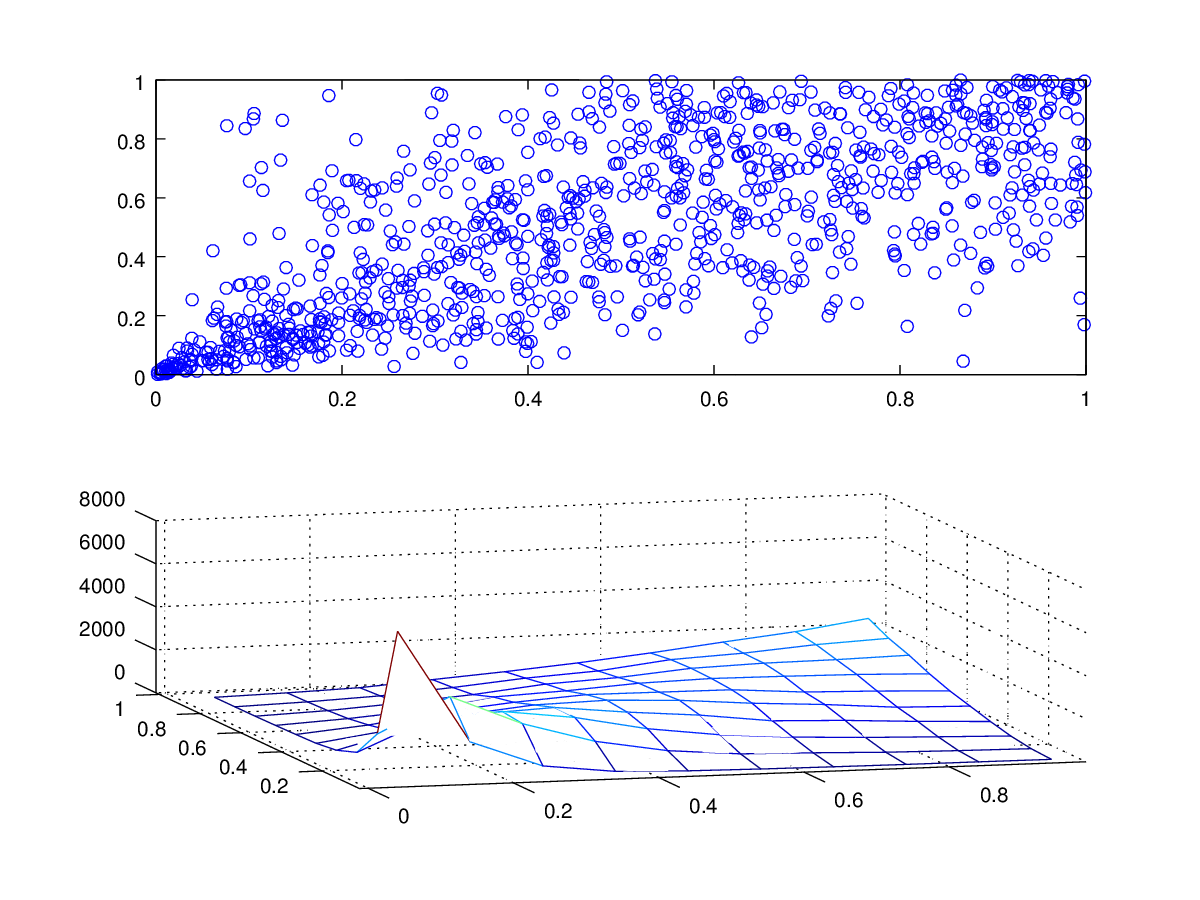
\includegraphics[scale = 0.50]{pictures/clayton.eps}
\caption{Dvourozměrná Claytonova kopula funkce s parametrem $\theta = 2$}
\end{figure}

Pro kalibraci Claytonovy kopula funkce stačí odhadnout parametr $\theta$. Mezi $\theta$ a Kendall pořadovou korelací $\rho_{\tau}$ existuje vztah
\begin{equation}
\rho_{\tau} = \frac{\theta}{\theta + 2}
\end{equation}
Prvním krokem kalibrace je tedy výpočet Kendall pořadové korelace (viz. výše), na který navazuje výpočet parametru $\theta$ pomocí inverze (2.2). Příslušná funkce \textit{FitClaytonCopula.m} je k dispozici v adresáři \textit{Copulas}.

Simulace z Claytonovy kopule probíhá v následujících krocích.
\begin{enumerate}
\item Vygenerujeme náhodnou veličinu $V \sim Ga(1/\theta, 1)$, kde $\theta > 0$ a $Ga(\alpha, \beta)$ je pravděpodobnostní rozdělení gamma s hustotou pravděpodobnosti
\begin{equation*}
f(x) = \frac{\beta^{\alpha}}{\Gamma(\alpha)}x^{\alpha - 1}e^{-\beta x}, ~~~ x > 0, \alpha > 0, \beta > 0
\end{equation*}
kde $\Gamma(\alpha) = \int_0^{\infty} x^{\alpha - 1}e^{-x}dx, ~~~ \alpha > 0$. Distribuční funkce náhodné veličiny $V$ má Laplace transformaci $\hat{G}(t) = (1 + t) ^ {-\frac{1}{\theta}}$.
\item Vygenerujeme nezávislé uniformní náhodné veličiny $X = (X_1, X_2)$.
\item Vypočteme $U = \left(\hat{G}(-\ln(X_1)/V), \hat{G}(-\ln(X_2)/V)\right)$. Dvourozměrný náhodný vektor $U$ je výběrem z Claytonovy kopula funkce.
\end{enumerate}
Funkci \textit{SimulClaytonCopula.m} pro simulaci z Clayton kopula funkce naleznete v adresáři \textit{Copulas}.

\subsubsection{Gumbelova kopula funkce}

Dvourozměrná Gumbelova kopula funkce má tvar
\begin{equation*}
C_{\theta}(u_1, u_2) = e^{-\left((-\ln(u_1))^{\theta} + (-\ln(u_2))^{\theta}\right)^{\frac{1}{\theta}}}, ~~~ 1 \le \theta < \infty
\end{equation*}
Jestliže $\theta = 1$, získáme nezávislou kopula funkci; jestliže $\theta \rightarrow \infty$, získáme komonotonickou kopula funkci. Parametr $\theta$ tak stejně jako v případě Claytonovy kopula funkce vyjadřuje míru závislosti.

\begin{figure}[htp]
\centering
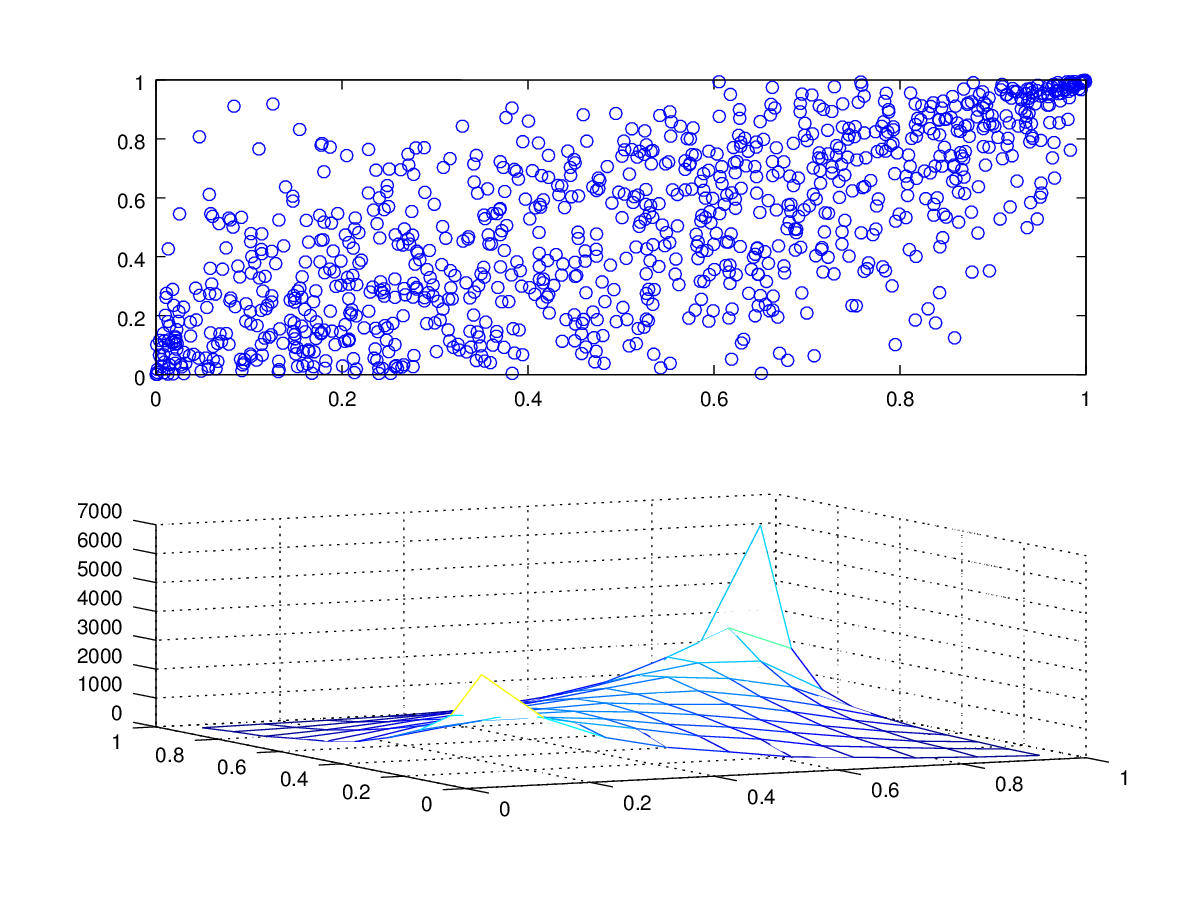
\includegraphics[scale = 0.50]{pictures/gumbel.eps}
\caption{Dvourozměrná Gumbelova kopula funkce s parametrem $\theta = 2$}
\end{figure}

Gumbelova kopula funkce je plně definována parametrem $\theta$. Stejně jako v případě Claytonovy kopula funkce existuje vztah mezi parametrem $\theta$ a Kendall pořadovou korelací $\rho_{\tau}$.
\begin{equation*}
\rho_{\tau} = \frac{\theta}{\theta + 2}
\end{equation*}
Pro kalibraci tedy nejprve stačí vypočíst Kendall pořadovou korelaci a z ní následně odvodit parametr $\theta$. Potřebná funkce \textit{FitGumbelCopula.m} je k dispozici v adresáři \textit{Copulas}.

Simulace sleduje podobné kroky jako v případě Claytonovy kopula funkce.
\begin{enumerate}
\item Vygenerujeme stabilní náhodnou veličinu $V \sim St(1 / \theta, 1, \gamma, 0)$, kde $\gamma = (cos(\pi/2\theta))^{\theta}$ a $\theta > 0$. Distribuční funkce náhodné veličiny $V$ má Laplace transformaci $\hat{G}(t) = e^{-t^{1/\theta}}$.
\item Vygenerujeme nezávislé uniformní náhodné veličiny $X = (X_1, X_2)$.
\item Vypočteme $U = \left(\hat{G}(-\ln(X_1)/V), \hat{G}(-\ln(X_2)/V)\right)$. Dvourozměrný náhodný vektor $U$ je výběrem z Gumbelovy kopula funkce.
\end{enumerate}

\subsubsection{Frankova kopula funkce}

Dvourozměrná Frankova kopula funkce má tvar
\begin{equation*}
C_{\theta}(u_1, u_2) = -\frac{1}{\theta}\ln \left(1 + \frac{(e^{-\theta u_1} - 1)(e^{-\theta u_2})}{e^{-\theta} - 1} \right) ~~~ \theta \in R - \{0\}
\end{equation*}

\begin{figure}[htp]
\centering
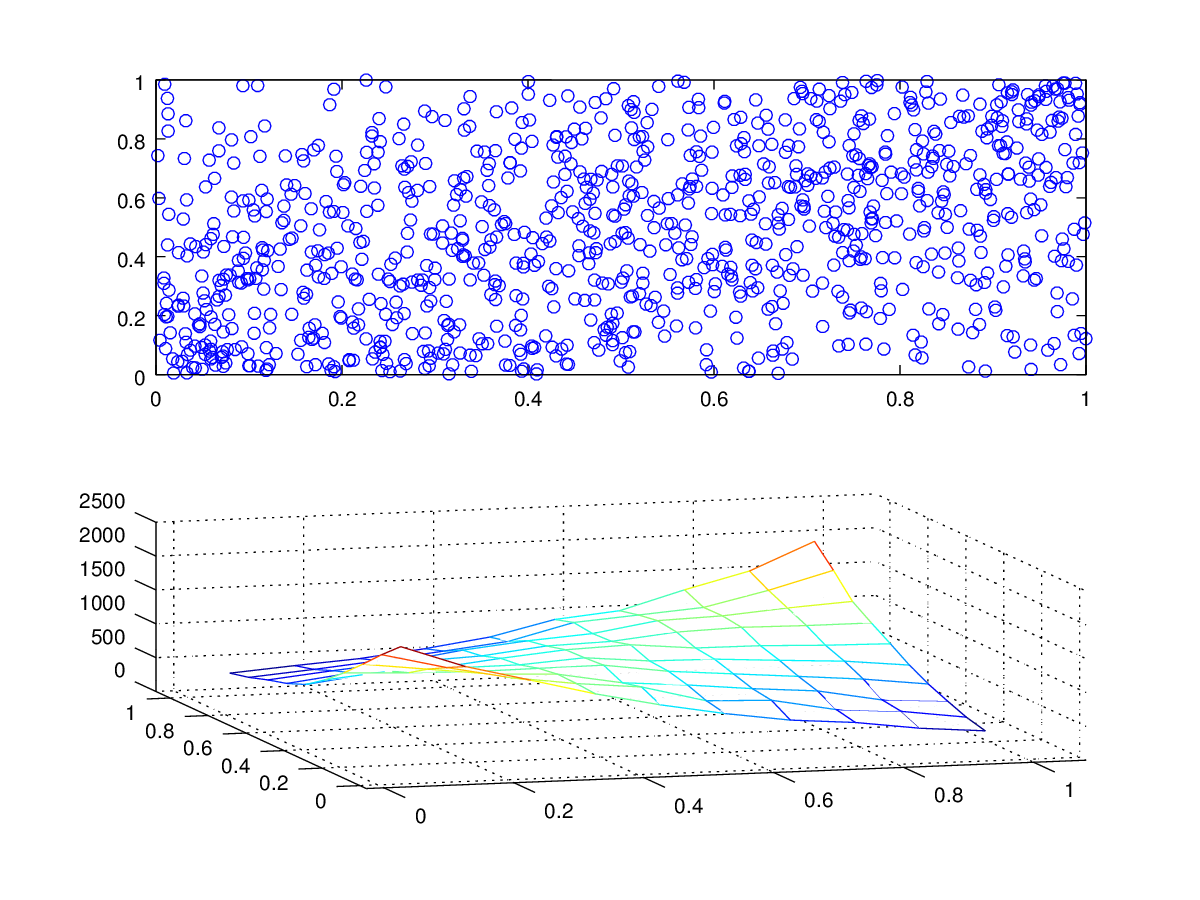
\includegraphics[scale = 0.50]{pictures/frank.eps}
\caption{Dvourozměrná Frankova kopula funkce s parametrem $\theta = 2$}
\end{figure}

Prvním krokem kalibrace Frankovy kopula funkce je výpočet Kendall pořadové korelace, ze které pomocí vztahu
\begin{equation*}
\rho_{\tau} = 1 - 4 \theta ^ {-1}\left(1 - D_1(\theta)\right)
\end{equation*}
kde $D_1(\theta) = \theta ^ {-1} \int_0^{\theta}\frac{t}{e^t - 1}dt$ je Debye funkce. Parametr $\theta$ nelze z tohoto vztahu vyjádřit přímo, a proto je třeba vypočíst iterativně např. pomocí Newtonovy metody.

Simulace z Frankovy kopula funkce probíhá v následujících krocích.
\begin{enumerate}
\item Vygenerujeme diskrétní náhodnou veličinu $V$ s pravděpodobnostní funkcí $p(k) = P(V = k) = \frac{(1 - e^{-\theta})^k}{k \theta}$ pro $k = 1, 2, ...$  a $\theta > 0$. Laplace transformace odpovídající distribuční funkce má tvar $\hat{G}(t) = \frac{1}{\theta} \ln \left(e^{-t}(1 - e^{-\theta}) - 1\right)$.
\item Vygenerujeme nezávislé uniformní náhodné veličiny $X = (X_1, X_2)$.
\item Vypočteme $U = \left(\hat{G}(-\ln(X_1)/V), \hat{G}(-\ln(X_2)/V)\right)$. Dvourozměrný náhodný vektor $U$ je výběrem z Frankovy kopula funkce.
\end{enumerate}
